% Options for packages loaded elsewhere
\PassOptionsToPackage{unicode}{hyperref}
\PassOptionsToPackage{hyphens}{url}
\PassOptionsToPackage{dvipsnames,svgnames,x11names}{xcolor}
%
\documentclass[
  12pt]{article}

\usepackage{amsmath,amssymb}
\usepackage{iftex}
\ifPDFTeX
  \usepackage[T1]{fontenc}
  \usepackage[utf8]{inputenc}
  \usepackage{textcomp} % provide euro and other symbols
\else % if luatex or xetex
  \usepackage{unicode-math}
  \defaultfontfeatures{Scale=MatchLowercase}
  \defaultfontfeatures[\rmfamily]{Ligatures=TeX,Scale=1}
\fi
\usepackage{lmodern}
\ifPDFTeX\else  
    % xetex/luatex font selection
\fi
% Use upquote if available, for straight quotes in verbatim environments
\IfFileExists{upquote.sty}{\usepackage{upquote}}{}
\IfFileExists{microtype.sty}{% use microtype if available
  \usepackage[]{microtype}
  \UseMicrotypeSet[protrusion]{basicmath} % disable protrusion for tt fonts
}{}
\makeatletter
\@ifundefined{KOMAClassName}{% if non-KOMA class
  \IfFileExists{parskip.sty}{%
    \usepackage{parskip}
  }{% else
    \setlength{\parindent}{0pt}
    \setlength{\parskip}{6pt plus 2pt minus 1pt}}
}{% if KOMA class
  \KOMAoptions{parskip=half}}
\makeatother
\usepackage{xcolor}
\setlength{\emergencystretch}{3em} % prevent overfull lines
\setcounter{secnumdepth}{5}
% Make \paragraph and \subparagraph free-standing
\makeatletter
\ifx\paragraph\undefined\else
  \let\oldparagraph\paragraph
  \renewcommand{\paragraph}{
    \@ifstar
      \xxxParagraphStar
      \xxxParagraphNoStar
  }
  \newcommand{\xxxParagraphStar}[1]{\oldparagraph*{#1}\mbox{}}
  \newcommand{\xxxParagraphNoStar}[1]{\oldparagraph{#1}\mbox{}}
\fi
\ifx\subparagraph\undefined\else
  \let\oldsubparagraph\subparagraph
  \renewcommand{\subparagraph}{
    \@ifstar
      \xxxSubParagraphStar
      \xxxSubParagraphNoStar
  }
  \newcommand{\xxxSubParagraphStar}[1]{\oldsubparagraph*{#1}\mbox{}}
  \newcommand{\xxxSubParagraphNoStar}[1]{\oldsubparagraph{#1}\mbox{}}
\fi
\makeatother


\providecommand{\tightlist}{%
  \setlength{\itemsep}{0pt}\setlength{\parskip}{0pt}}\usepackage{longtable,booktabs,array}
\usepackage{calc} % for calculating minipage widths
% Correct order of tables after \paragraph or \subparagraph
\usepackage{etoolbox}
\makeatletter
\patchcmd\longtable{\par}{\if@noskipsec\mbox{}\fi\par}{}{}
\makeatother
% Allow footnotes in longtable head/foot
\IfFileExists{footnotehyper.sty}{\usepackage{footnotehyper}}{\usepackage{footnote}}
\makesavenoteenv{longtable}
\usepackage{graphicx}
\makeatletter
\def\maxwidth{\ifdim\Gin@nat@width>\linewidth\linewidth\else\Gin@nat@width\fi}
\def\maxheight{\ifdim\Gin@nat@height>\textheight\textheight\else\Gin@nat@height\fi}
\makeatother
% Scale images if necessary, so that they will not overflow the page
% margins by default, and it is still possible to overwrite the defaults
% using explicit options in \includegraphics[width, height, ...]{}
\setkeys{Gin}{width=\maxwidth,height=\maxheight,keepaspectratio}
% Set default figure placement to htbp
\makeatletter
\def\fps@figure{htbp}
\makeatother

\addtolength{\oddsidemargin}{-.5in}%
\addtolength{\evensidemargin}{-1in}%
\addtolength{\textwidth}{1in}%
\addtolength{\textheight}{1.7in}%
\addtolength{\topmargin}{-1in}%
\makeatletter
\@ifpackageloaded{caption}{}{\usepackage{caption}}
\AtBeginDocument{%
\ifdefined\contentsname
  \renewcommand*\contentsname{Table of contents}
\else
  \newcommand\contentsname{Table of contents}
\fi
\ifdefined\listfigurename
  \renewcommand*\listfigurename{List of Figures}
\else
  \newcommand\listfigurename{List of Figures}
\fi
\ifdefined\listtablename
  \renewcommand*\listtablename{List of Tables}
\else
  \newcommand\listtablename{List of Tables}
\fi
\ifdefined\figurename
  \renewcommand*\figurename{Figure}
\else
  \newcommand\figurename{Figure}
\fi
\ifdefined\tablename
  \renewcommand*\tablename{Table}
\else
  \newcommand\tablename{Table}
\fi
}
\@ifpackageloaded{float}{}{\usepackage{float}}
\floatstyle{ruled}
\@ifundefined{c@chapter}{\newfloat{codelisting}{h}{lop}}{\newfloat{codelisting}{h}{lop}[chapter]}
\floatname{codelisting}{Listing}
\newcommand*\listoflistings{\listof{codelisting}{List of Listings}}
\makeatother
\makeatletter
\makeatother
\makeatletter
\@ifpackageloaded{caption}{}{\usepackage{caption}}
\@ifpackageloaded{subcaption}{}{\usepackage{subcaption}}
\makeatother
\ifLuaTeX
  \usepackage{selnolig}  % disable illegal ligatures
\fi
\usepackage[]{natbib}
\bibliographystyle{agsm}
\usepackage{bookmark}

\IfFileExists{xurl.sty}{\usepackage{xurl}}{} % add URL line breaks if available
\urlstyle{same} % disable monospaced font for URLs
\hypersetup{
  pdftitle={Zoning: A Barrier or Solution to Truck Parking Infrastructure Shortages?},
  pdfauthor={William Clinton Co},
  colorlinks=true,
  linkcolor={blue},
  filecolor={Maroon},
  citecolor={Blue},
  urlcolor={Blue},
  pdfcreator={LaTeX via pandoc}}


\begin{document}


\def\spacingset#1{\renewcommand{\baselinestretch}%
{#1}\small\normalsize} \spacingset{1}


%%%%%%%%%%%%%%%%%%%%%%%%%%%%%%%%%%%%%%%%%%%%%%%%%%%%%%%%%%%%%%%%%%%%%%%%%%%%%%

\date{April 17, 2025}
\title{\bf Zoning: A Barrier or Solution to Truck Parking Infrastructure
Shortages?}
\author{
William Clinton Co\thanks{I am grateful to Professor Terry Moon for
their invaluable guidance and advice, and to Professor Ron Yang for his
mentorship and support in my academic development. I also thank my
classmates in UBC's ECON 490 class for their insightful feedback, which
helped improve this paper.}\\
Department of Economics, University of British Columbia\\
}
\maketitle

\bigskip
\bigskip
\begin{abstract}
Truck parking shortages across North America exacerbate accident risk.
We merge three novel datasets, FMCSA crash reports, Puentes et al.'s
(2006) zoning classifications, and Yang's (2024) geocoded truck stop
openings, to examine whether restrictive zoning regimes inhibit the
supply-side response to severe truck-parking accidents. Using
county‑year panels from 2000--2016, we implement (i) a fixed‑effects
model exploiting pre‑2007 variation in high‑severity, parked‑truck
crashes to predict truck-stop growth (2006--2016), and (ii) a
difference‑in‑differences design leveraging 2007--2015 accident shocks
to compare treated versus control jurisdictions.Our results show that
jurisdictions experiencing high-severity parked-truck accidents tend to
build significantly more truck stops over the following decade,
suggesting a decentralized, demand-responsive adjustment mechanism.
However, this pattern is not consistent across all states, some exhibit
a muted response. While local markets often respond to safety signals,
targeted state-level interventions may be necessary in structurally
constrained states to improve freight safety and efficiency.
\end{abstract}


\newpage
\spacingset{1.9} % DON'T change the spacing!

\section{Introduction}\label{introduction}

Truck parking shortages in North America contribute to higher accident
rates, increased costs, delayed goods, and reduced public safety. With
trucks delivering 80\% of goods, the infrastructure has not kept pace
with industry growth. Approximately 43.8\% to 98\% of the 3.87 million
truck drivers in the U.S. and Canada face parking challenges, spending
an average of 56 minutes daily searching for parking. This inefficiency
results in an estimated \$5,600 annual loss per driver, totaling about
\$21.69 billion nationwide. Additionally, restrictive zoning laws,
enforced by over 90,000 local governments, hamper the development of new
truck parking facilities, as local opposition often stems from land
value concerns and public resistance.

Existing studies on zoning provide valuable context but are limited in
scope. Research often focuses on single areas (Chicago, Eastern
Massachusetts) and are often focused on aspects unrelated to truck
zoning regulation
\citep{shertzerRaceEthnicityDiscriminatory2016, glaeserCausesConsequencesLand2009}
or are scoped in international contexts such as Brazil
\citep{anagolEstimatingEconomicValue2021}. Furthermore, most literature
emphasizes US residential zoning
\citep{lensStrictLandUse2016, huangResidentialLandUse2012}or office
space \citep{cheshireOfficeSpaceSupply2008}, leaving industrial zoning
and its implications for truck parking largely unexplored. All of these
papers demonstrate that zoning reforms are binding and limit overall
population welfare in favor of benefiting a select few.

Initially designed to balance public welfare and economic development,
zoning regulations have evolved, sometimes adapting to market forces or
catering to local stakeholder interests, such as middle-class homeowners
\citep{fischelEconomicHistoryZoning2024}. While zoning has the potential
to enhance economic productivity, it can also introduce inefficiencies,
particularly in industrial applications
\citep{mcdonaldPDFEconomicsZoning2012}. Fragmented zoning governance
often discourages communities from accommodating truck parking, despite
its regional benefits, due to localized decision-making dynamics.
Furthermore, it is unclear whether the current state of land regulation
optimizes welfare. Some estimates say misallocation through zoning
welfare cost the economy up to 13.6 percent of gross domestic product
\citep{osmanRestrictiveLandUse2020}. This paper aims to address this gap
within the context of truck parking shortages these challenges. Previous
research, such as \citet{liangSafetyInspectionsImprove2021}, has
utilized similar datasets to examine the impact of safety inspections on
crash rates. Our study builds on this foundation by integrating
additional spatial and regulatory dimensions, providing a more
comprehensive understanding of the factors influencing truck-related
accidents.

This methodology has not been explored before primarily due to data
limitations and the recent emergence truck infrastructure issues. For
instance the landmark legislation, Jason's Law, only came into effect in
2012. The rise of e-commerce, coupled with aging populations and
increasing NIMBY-ism, has exacerbated supply chain challenges in recent
years. Furthermore, the data has only recently become available. This
unique data set and the recency of the issue make our study a novel
empirical contribution to the field. This paper investigates whether
restrictive zoning regimes inhibit the supply-side response to severe
truck parking accidents by limiting subsequent growth in truck stop
infrastructure.

To identify causal effects, we implement two empirical strategies.
First, a fixed effects specification exploits variation in accident
timing and severity to estimate the association between cumulative
pre-2007 accident exposure and truck stop growth from 2006 to 2016,
controlling for zoning category, region, and year fixed effects. Second,
a difference-in-differences (DiD) design uses accidents between 2007 and
2015 as treatment shocks, comparing post-treatment changes in treated
versus control locations, conditional on zoning and fixed effects. Both
strategies assume exogeneity in accident timing and location, and a
unidirectional relationship where accidents drive infrastructure
response, not vice versa.

Our identification strategy is supported by pre-trend validation and
region-level clustering to account for spatial correlation in trucking
activity and infrastructure. The data combines: (1) FMCSA crash reports
(1993--2016) for treatment events; (2) zoning classifications from
Puentes et al.~(2006) to proxy regulatory restrictiveness; and (3)
Yang's (2024) truck stop directory, which identifies truck stop openings
by year and location. The analysis sample is a jurisdiction-year panel
(2000--2016) matched across datasets.

Together, these methods allow us to isolate the extent to which zoning
regimes mediate the infrastructure response to safety-driven demand
shocks, providing new evidence on how land-use regulation interacts. The
main result is that treatment jurisdictions, those with high-severity
parked-truck accidents, experienced a significant increase in truck stop
growth. DiD estimates show a statistically and economically significant
increase in truck stop count. This paper finds that local jurisdictions
generally respond to severe parked-truck accidents by expanding truck
stop infrastructure, suggesting a decentralized, demand-responsive
adjustment mechanism. These results imply that widespread federal or
state-level mandates may be unnecessary, as local markets often
internalize safety signals and adjust capacity accordingly. However, the
study also identifies persistent truck stop shortages in several states,
such as California, Nevada, New York, New Jersey, Mississippi, and
Oregon, where restrictive zoning, geographic constraints, or
institutional barriers may inhibit such market-driven responses. In
these outlier cases, targeted policy interventions may be warranted to
overcome entrenched limitations and improve safety outcomes.

Overall, the evidence supports a differentiated policy approach, allow
local flexibility where markets function well, but intervene selectively
in structurally constrained corridors. Future research should further
investigate the institutional and regulatory heterogeneity that shapes
these differential responses to demand shocks in critical
infrastructure.

\section{Institutional Setting}\label{institutional-setting}

The Federal Motor Carrier Safety Administration (FMCSA), maintains a
comprehensive database known as the Crash File. This dataset records all
reported motor vehicle crashes in the United States, providing detailed
insights into the nature and conditions of each accident. Key attributes
include the type of vehicle involved (e.g., trucks, motorcycles, or
buses), the circumstances of the crash (e.g., involving a parked
vehicle), the number of vehicles involved, any fatalities or injuries,
and relevant weather conditions, and observations. Our data is
(1990-Present) FMCA Crash file from USDOT
(\phantomsection\label{sec:appendix-a}\hyperref[sec-a.-visualization-of-dataset.-]{Appendix
A}).

Our dataset spans from 1990 to the present, with a focus on records from
1993 to 2016. A unique feature of this dataset is its ability to
distinguish trucks as a specific variable, allowing for a granular
analysis of truck-involved collisions. Furthermore, it offers detailed
information on accident circumstances, such as whether a truck was
illegally parked, a distinction not commonly found in other datasets.

We also incorporate a digitized data set tracking truck stop creation
from 2006 to 2016. This data set enables us to analyze the impact of new
truck stops on accident patterns at the county level. Notably, this
period lacks significant policy reforms or major events that could
confound our analysis. We refine our analysis by incorporating zoning
classifications from \citet{puentesTraditionalReformedReview2006}
(\hyperref[sec-b.-map-of-zoning-categories]{B. Map of Zoning
Categories}), which categorize land use regulations into four distinct
zoning types. These classifications serve as fixed effects in our study.
We study high accidents events and their effect on truck stop creation,
with zoning category fix effect, in order to study our research
question.

\section{Empirical Strategy \& Data
Sources}\label{empirical-strategy-data-sources}

This paper investigates whether restrictive zoning environments inhibit
truck stop growth following fatal parked-truck accidents. We test this
using two empirical strategies: a fixed effects model and a
difference-in-differences (DiD) design, leveraging variation in zoning
regimes and accident timing. The underlying causal chain motivating our
approach is:

Insufficient Truck Parking → Illegal Truck Parking → \emph{Accidents} →
Increased Demand → \emph{Truck Stop Growth}

\subsection{Fixed Effects
Specification}\label{fixed-effects-specification}

Our first approach estimates the relationship between cumulative severe
truck parking-related accidents and subsequent truck stop growth,
controlling for location characteristics and time shocks. The estimating
equation is:

\[
\Delta \text{NumTruckStop}_{jlt} = \sum_{i=1993}^{2006} \text{Fatality}_{jli} + \gamma_j + \lambda_t + \mu_l + \epsilon_{jlt}
\]

The estimating equation examines how severe parked-truck accidents
influence changes in truck stop infrastructure. The dependent variable,
\(\Delta \text{NumTruckStop}_{jlt}\), is the change in the number of
truck stops from 2006 to 2016 in zoning category \(j\), location \(l\),
and year \(t\). The main explanatory variables are indicators for
high-fatality parked-truck accidents, \(\text{Fatality}_{jli}\),
occurring from 1993 to 2006. An accident is considered high-severity if
its severity exceeds two standard deviations above the mean. The model
includes zoning fixed effects (\(\gamma_j\)), year fixed effects
(\(\lambda_t\)), and regional fixed effects (\(\mu_l\)).

This model uses pre-2007 accident data to predict post-2006
infrastructure changes. The assumption is that accident timing and
severity are exogenous and uncorrelated with omitted drivers of truck
stop growth. The zoning categories, Traditional, Exclusion, Reform, and
Wild Wild Texas, included as fixed effects, assumed non-collinear and
independent across jurisdictions.

Our identification assumption is that in areas lacking legal truck
parking, drivers resort to illegal options, increasing accident risk. In
response to visible safety concerns, localities are pressured to
increase legal truck parking, reflected in new truck stops. This logic
supports a one-way causal structure: accidents prompt infrastructure,
not vice versa.

To capture regional heterogeneity in trucking activity, regulation, and
climate, we cluster standard errors at the region level. Clustering
standard errors by region assumes that observations within a region may
be correlated, while observations across regions are independent. This
accounts for potential intra-regional shocks or unobserved factors that
could bias standard errors if ignored. This accounts for spatial
correlation in accident rates and infrastructure trends, ensuring robust
inference.

\subsection{Difference-in-Differences (DiD)
Design}\label{difference-in-differences-did-design}

To complement and alleviate some of the limitations (reverse causality)
of the fixed effects approach, we implement a DiD model using accidents
from 2007 to 2015 as quasi-random treatment shocks:

\[
\Delta \text{NumTruckStop}_{lt} = \sum_{i \in \{2007, ..., 2016\}} \text{Accident}_{lt=i} + \gamma_j + \lambda_t + \mu_l + \epsilon_{jlt}
\]

Here, \(\text{Accident}_{jlt}\) is a binary indicator for whether a
high-severity parked-truck accident occurred in location \(l\), zoning
category \(j\), in year \(t\). The model compares post-treatment
outcomes in affected versus unaffected jurisdictions, conditioning on
location, year, and zoning fixed effects.

The DiD strategy relies on a parallel trends assumption: in the absence
of accidents, treated and untreated areas would follow similar
trajectories in truck stop development. We assess this by checking
pre-treatment trends across groups. If pre-2007 truck stop growth is
similar across accident exposure groups, we interpret post-treatment
differences as causal effects.

By definition, places also can not anticipate accidents. We also assume
that accident timing is unrelated to long-term planning efforts, and
that events in one region do not influence truck stop development in
adjacent regions. Each region's treatment status is assumed to impact
only its own infrastructure trajectory.

As with the fixed effects model, we cluster standard errors at the
regional level to address within-region correlation.

Our treatment variable is derived from the FMCSA crash database, which
documents all reportable truck crashes across the United States. For
this study, we use a cleaned panel spanning approximately 1993 to 2016,
focusing specifically on incidents involving parked trucks. The dataset
includes indicators of crash severity and fatalities, which serve as
proxies for truck parking demand. To capture variation in land use
regulation, we adopt the zoning typology developed by Puentes, Martin,
and Pendall (2006) \citep{puentesTraditionalReformedReview2006}, which
classifies jurisdictions into four categories: \emph{Traditional}
(rigid, legacy codes), \emph{Exclusion} (suburban and restrictive),
\emph{Reform} (modernized and flexible), and \emph{Wild Wild Texas}
(minimal or no formal zoning). These classifications allow us to capture
regulatory heterogeneity across regions. To measure supply-side
responses, we use Yang's (2024) geocoded directory of truck stop
establishments. Although the dataset is limited to a subset of years,
specifically 2006, 2007, 2008, 2014, 2015, and 2016, it provides
detailed information on truck stop locations and opening years. This
enables us to construct a panel of truck stop counts at the county level
and examine how infrastructure evolves over time in response to safety
shocks.

\section{Results and Economics
Interpretation}\label{results-and-economics-interpretation}

Figure~\ref{fig-SummaryTable} presents the estimated coefficients from
the fix effects model analyzing the relationship across four
specifications. The reference period is 2006--2007.

The high-fatality crash interaction terms show consistently positive and
significant coefficients. The strongest effects appear in the 2002--2003
period, with coefficients of 2.384*** (Model 1) to 3.466*** (Model 4),
indicating localities built 2.4-3.5 more truck stops over the following
decade compared to the reference period. This 5-year lag matches typical
infrastructure timelines. Results remain robust across specifications,
with RMSE declining from 1.72 to 1.41 as fixed effects are added.

\begin{figure}

\centering{

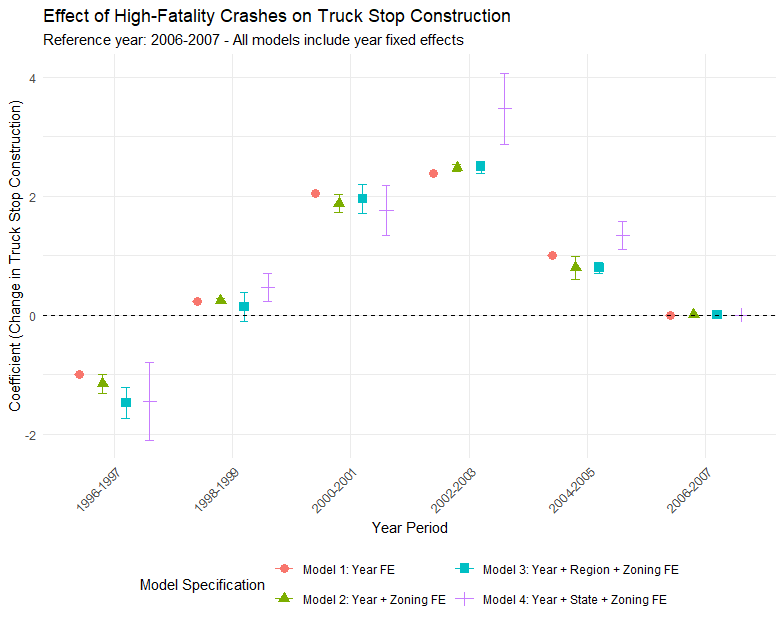
\includegraphics[width=5.67708in,height=\textheight]{images/Rplot.png}

}

\caption{\label{fig-time}Time Coefficients of Event Study Model}

\end{figure}%

\begin{figure}

\centering{

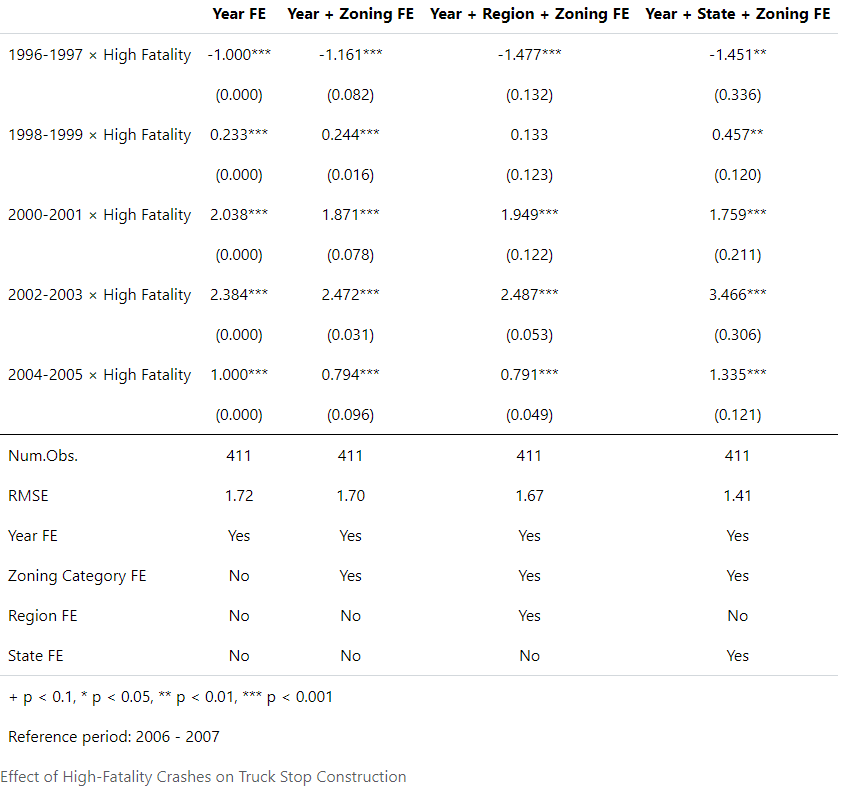
\includegraphics[width=5.59375in,height=\textheight]{images/Screenshot 2025-03-09 225540.png}

}

\caption{\label{fig-SummaryTable}Summary Table of Time Coefficients}

\end{figure}%

Figure~\ref{fig-zoning_table} and Figure~\ref{fig-zonign_categories}
present coefficient estimates for zoning categories across three model
specifications, with Wild Texas as the reference zoning category. Zoning
categories show minimal explanatory power, with coefficients for
Exclusion, Reform, and Wild Texas zones remaining statistically
insignificant across specifications. The marginally significant effects
that appear (Exclusion: 0.740+, p\textless0.1 in Model 2; Reform:
-0.540+, p\textless0.1 in Model 1) disappear when controlling for
spatial heterogeneity, suggesting zoning regulations play a negligible
role in construction outcomes relative to regional or state-level
factors.

\begin{figure}

\centering{

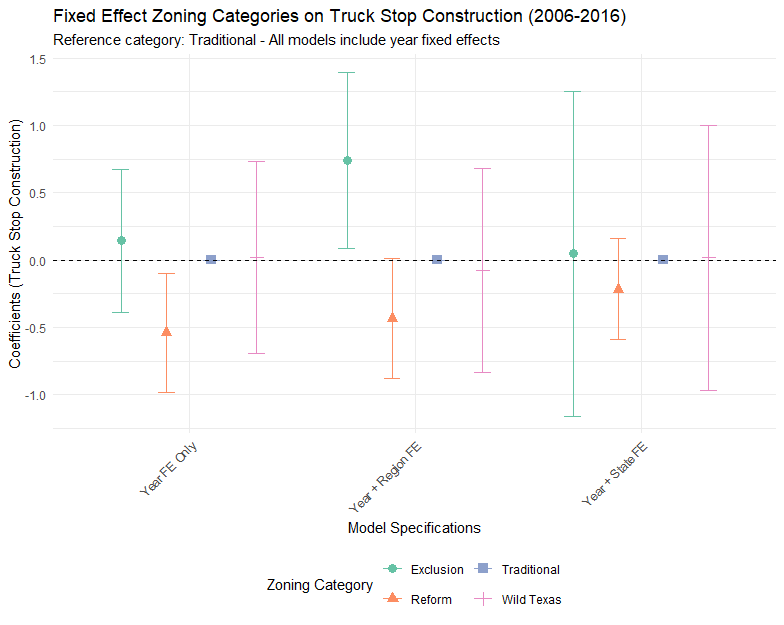
\includegraphics[width=6.01042in,height=\textheight]{images/Rplot01.png}

}

\caption{\label{fig-zonign_categories}Zoning Category Coefficients Plot}

\end{figure}%

\begin{figure}

\centering{

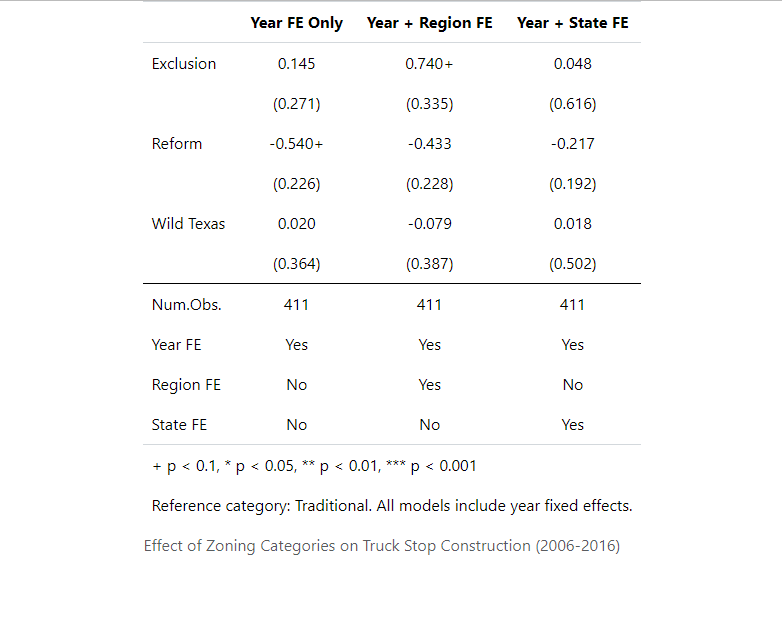
\includegraphics[width=5.78125in,height=\textheight]{images/Rplot05.png}

}

\caption{\label{fig-zoning_table}Zoning Category Coefficients Table}

\end{figure}%

Figure~\ref{fig-StateZoning} presents the estimated state fixed effects
on truck stop construction between 2006 and 2016, with North Dakota
serving as the reference category. The coefficients represent deviations
from the median effect, accounting for year fixed effects. States with
significantly positive coefficients, such as Illinois and Arizona, show
an associated increase in truck stop construction following parking
accidents, typically by two additional facilities.

\begin{figure}

\centering{

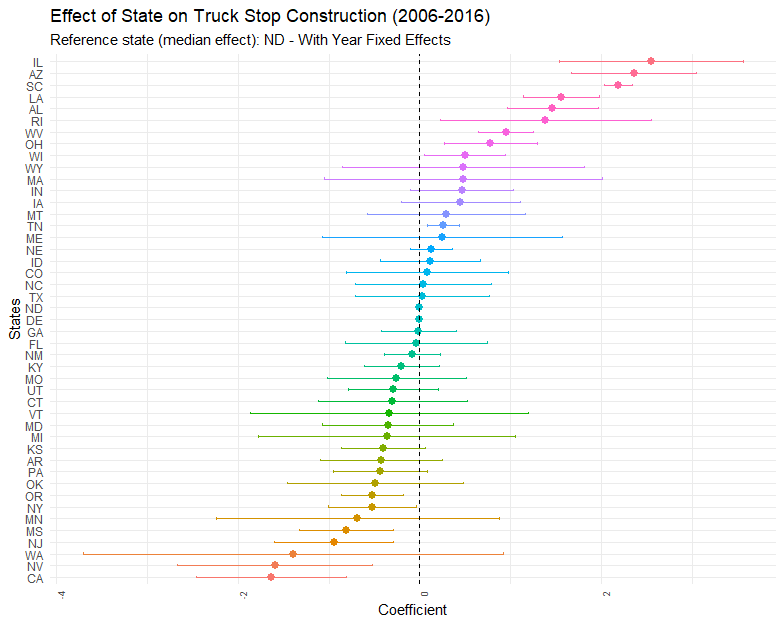
\includegraphics[width=6.19792in,height=\textheight]{images/Rplot04.png}

}

\caption{\label{fig-StateZoning}Coefficient of State Fix Effect}

\end{figure}%

Section~\ref{sec-parallel-trends-chart-fixed-effect-model} shows
counties with pre-2006 high-fatality accidents consistently built more
truck stops, aligning with infrastructure needs.
Section~\ref{sec-parallel-trends-chart-did-model} confirms parallel
pre-treatment trends (2008-2015), with post-2015 divergence (+0.6 annual
change in accident-prone counties). This supports a interpretation: the
increase stems from post-accident responses, not pre-existing trends.
Non-parallel trends bias appears unlikely.

Our DiD estimates (Figure~\ref{fig-did}, Figure~\ref{fig-DID_table})
compare locations with high-fatality accidents (2008-2015) to controls
(no accident) across four specifications. Models with zoning, region,
and state fixed effects show consistent estimates (adj. R²:
0.005-0.015). The 2015 coefficient exhibits a statistically significant
positive value , indicating that jurisdictions responded to
high-fatality accidents occurring between 2008-2015 by constructing
additional truck stops, relative to the baseline. Balancing tests
(\hyperref[sec-c.-balancing_chart_region]{C. Balancing Chart},
\hyperref[sec-D.balancing_chart_state]{D. Balancing Chart}) confirm
parallel pre-trends, supporting our design.

\begin{figure}

\centering{

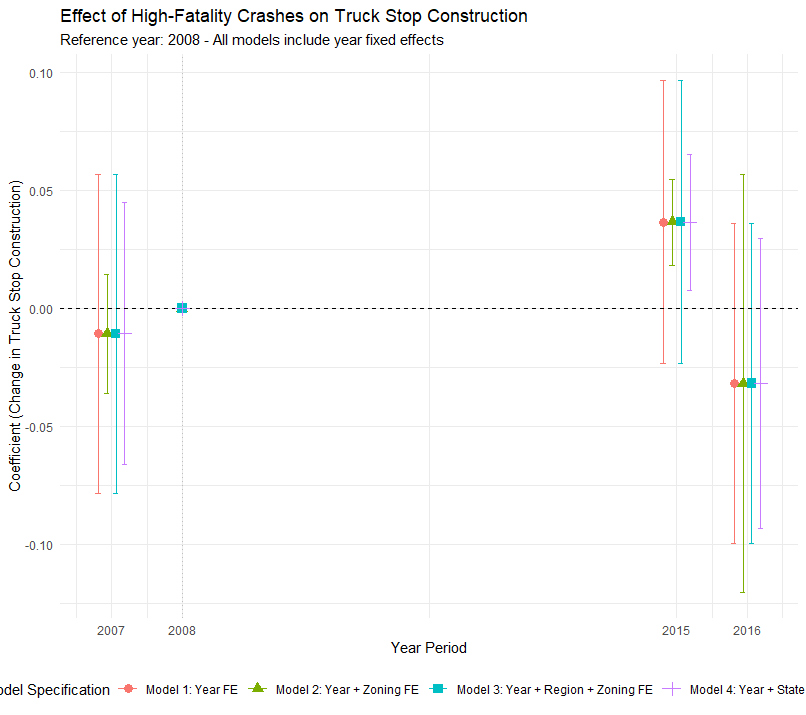
\includegraphics{images/Rplot07-01.png}

}

\caption{\label{fig-did}Coefficients of DID Model}

\end{figure}%

\begin{figure}

\centering{

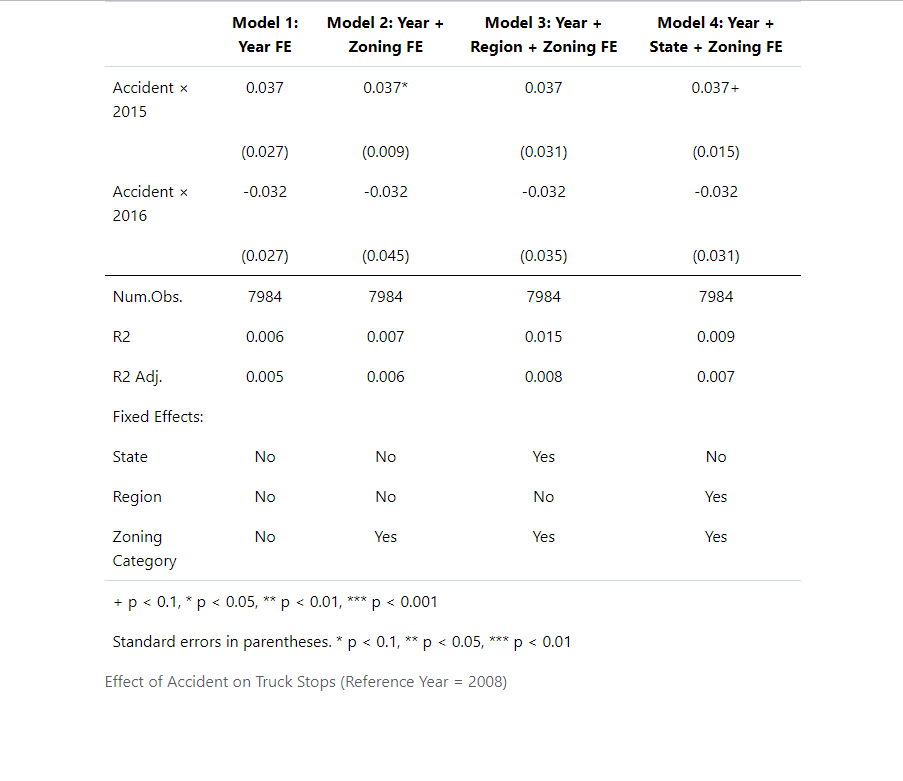
\includegraphics{images/clipboard-2216259381.png}

}

\caption{\label{fig-DID_table}Results of DID Model}

\end{figure}%

Figure~\ref{fig-DID_FE_categories} presents coefficient estimates for
zoning categories across three model specifications, using ``Wild
Texas'' as the reference. The results are consistent with our baseline
fixed-effects models, suggesting that zoning plays a limited role in
truck stop construction. Most categories have small, statistically
insignificant effects. While the ``Exclusion'' category shows a
significant coefficient in some models, its sign varies, likely due to
limited sample size, so we interpret it with caution. Overall, zoning
does not appear to strongly mediate jurisdictional responses to trucking
accidents. Prior work has focused on broader infrastructure or land use
impacts on housing, leaving no directly comparable estimates.

\begin{figure}

\centering{

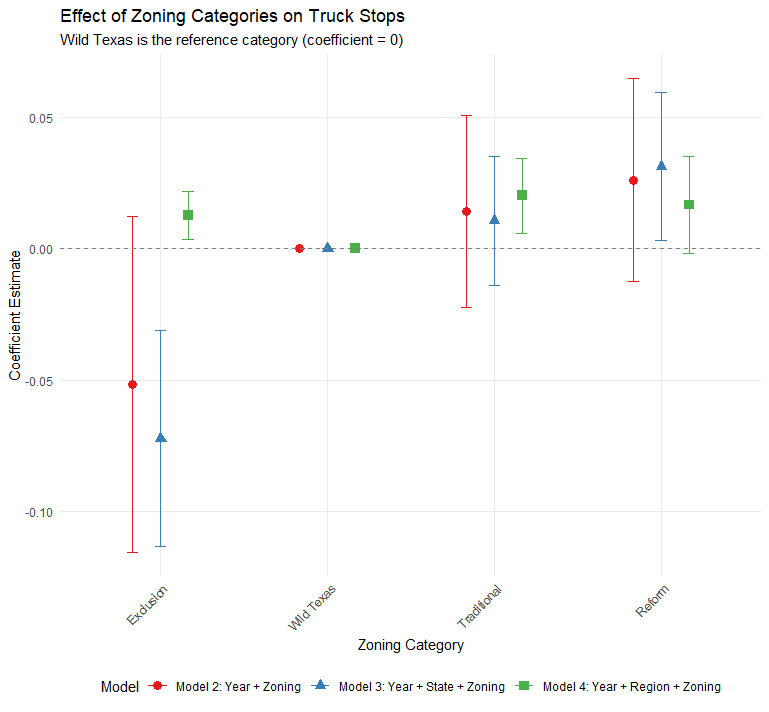
\includegraphics{images/clipboard-3981034325.png}

}

\caption{\label{fig-DID_FE_categories}Zoning Coefficients of DID model}

\end{figure}%

\subsection{Bias}\label{bias}

Our estimates may understate the true effect of high-fatality truck
crashes on truck infastructure construction responses. This downward
bias could stem from unobserved capacity expansions at existing truck
stops, which our data, limited to new construction, not capture. Zoning
classifications, which tend to be stable and self-reinforcing over time
\citep{mclaughlinLandUseRegulation2012}, may further discourage new
development, compounding the bias. Our analysis may understate the true
effect if jurisdictions preemptively address infrastructure needs
through policy changes (e.g., parking or traffic regulations), biasing
estimates downward. Other factors, such as unobserved policy responses
or lobbying, may also influence results, though their direction is
unclear. Finally, the concentration of accidents around 2007 and 2015,
along with limited data outside this window, restricts our ability to
generalize findings, nor analyze the underlying truck stop construction
outside these years, which adds uncertainty to our results. Broader,
longitudinal data would help validate and extend our conclusions. It
would allow us to explore and validate our unidirectional causality,
addressing potential reverse causality limitations.

\section{Policy Implication and
Conclusion}\label{policy-implication-and-conclusion}

The findings suggest that most localities self-regulate truck stop
supply in response to safety concerns, with new truck stops often
established following severe accidents. This market-driven response
indicates that broad federal or state interventions may be unnecessary.
Instead, local actors appear to address capacity constraints as they
arise.

However, persistent shortages in states like California, Nevada, New
York, New Jersey, Mississippi, and Oregon point to deeper structural
barriers (Figure~\ref{fig-StateZoning}). These states may benefit from
targeted policy support to overcome regulatory or geographic
constraints. While zoning effects are generally limited, localized
reforms in high-demand corridors could improve freight safety.

In sum, truck stop shortages are often addressed locally, but selective
state-level action is warranted where systemic barriers remain. Targeted
investment in these areas can enhance road safety and support efficient
freight movement.

Future research could expand on this work by analyzing institutional
contexts, such as state DOT policies or municipal zoning boards, to
explain local response variation. Testing results with alternative
accident severity metrics or zoning measurements like the Wharton Land
Use Regulatory Index (WLIURA), whiel also considering placebo tests and
conditional zoning models. \citep{gyourkoNewMeasureLocal2008} may also
be valuable. More granular datasets, including the
\href{https://www.nhtsa.gov/file-downloads}{NHTSA File Downloads} and
\href{https://www.nhtsa.gov/research-data/fatality-analysis-reporting-system-fars}{Fatality
Analysis Reporting System (FARS)}, could improve measurement precision.
Additionally, incorporating insurance claims or
\href{https://data.transportation.gov/Trucking-and-Motorcoaches/Motor-Carrier-Crash-Data-/b8e5-isfj}{Motor
Carrier Crash Data} from the U.S. DOT, along with more detailed state
DOT datasets (e.g., Texas), could provide deeper insights into accident
causes and their relation to policy responses.

\section{\texorpdfstring{\textbf{Appendix}}{Appendix}}\label{appendix}

\subsection{Remark: Scale of Truck Parking Challenges
vs.~Homelessness}\label{remark-scale-of-truck-parking-challenges-vs.-homelessness}

While homelessness remains a serious social concern in North America,
the shortage of truck parking affects an even larger population. With
approximately 3.5 million truck drivers in the U.S. and Canada, the
Federal Highway Administration (FHWA) estimates that 43.8\%, or about
1.53 million drivers, struggle to find safe, adequate parking. Other
sources, such as the American Transportation Research Institute (ATRI)
and the U.S. Department of Transportation (USDOT), estimate the figure
to be as high as 70\%--98\%.

In contrast, the combined homeless population of the U.S.
(\textasciitilde580,000), Canada (\textasciitilde235,000), and Mexico
(\textasciitilde50,000) totals around 865,000. Even using the
conservative FHWA estimate, the truck parking shortage affects nearly
twice as many individuals.

Both crises deserve attention, but in terms of scale, the truck parking
shortage rivals, if not exceeds, the homelessness crisis across North
America.

\subsection{\texorpdfstring{\textbf{Visualization of
dataset.}}{Visualization of dataset.}}\label{sec-a.-visualization-of-dataset.-}

(Present Truck stop parking observatios also available
\href{https://data-usdot.opendata.arcgis.com/datasets/usdot::truck-stop-parking/about}{Truck
Stop Parking \textbar{} Geospatial at the Bureau of Transportation
Statistics})

\begin{figure}[H]

{\centering 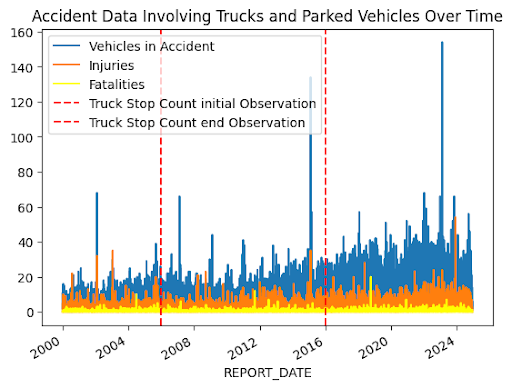
\includegraphics[width=4.27083in,height=\textheight]{images/unnamed.png}

}

\caption{Dataset Visualization}

\end{figure}%

\subsection{Map of Zoning
Categories}\label{sec-b.-map-of-zoning-categories}

\begin{figure}[H]

{\centering 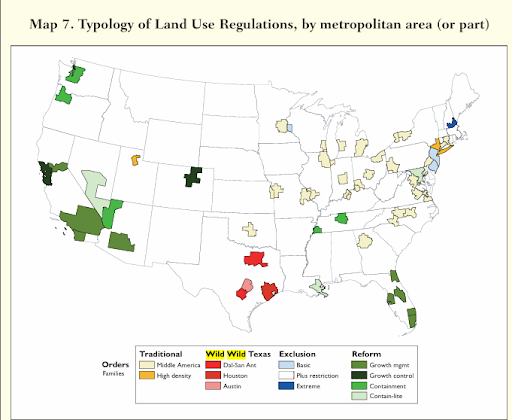
\includegraphics{images/unnamed (1).png}

}

\caption{Zoning Category Map}

\end{figure}%

\subsection{Balancing Chart
(Region)}\label{sec-c.-balancing_chart_region}

\begin{figure}[H]

{\centering 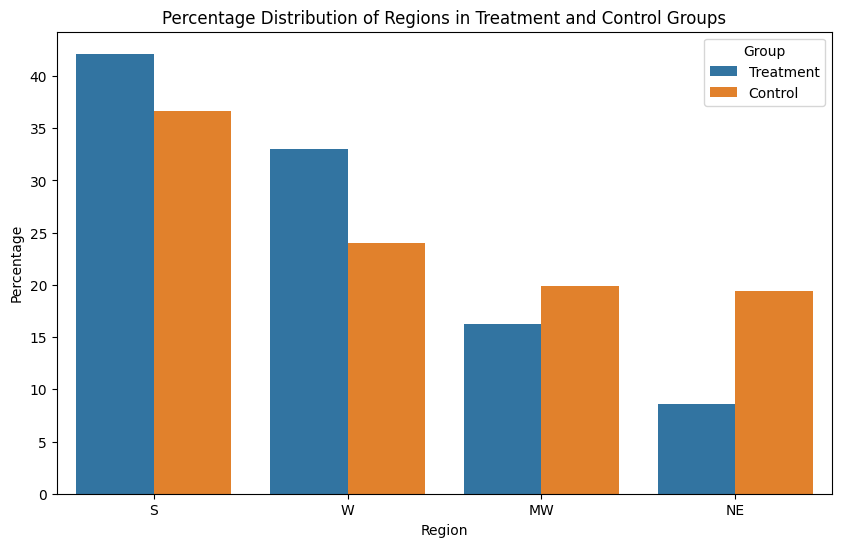
\includegraphics{images/clipboard-2848566608.png}

}

\caption{Balancing Chart Region}

\end{figure}%

\subsection{Balancing Chart (State)}\label{sec-D.balancing_chart_state}

\begin{figure}[H]

{\centering 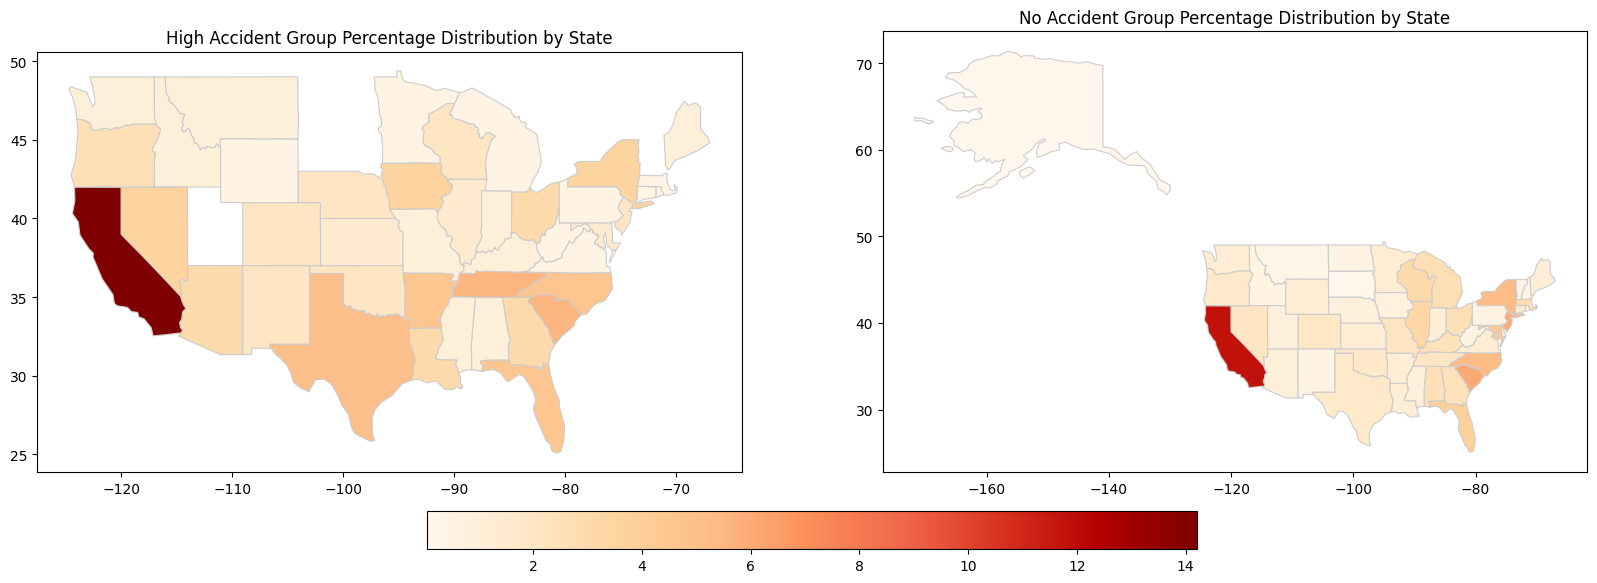
\includegraphics{images/clipboard-2792065255.png}

}

\caption{Balancing Chart State}

\end{figure}%

\subsection{Parallel Trends Chart Fixed Effect
Model}\label{sec-parallel-trends-chart-fixed-effect-model}

\begin{figure}[H]

{\centering 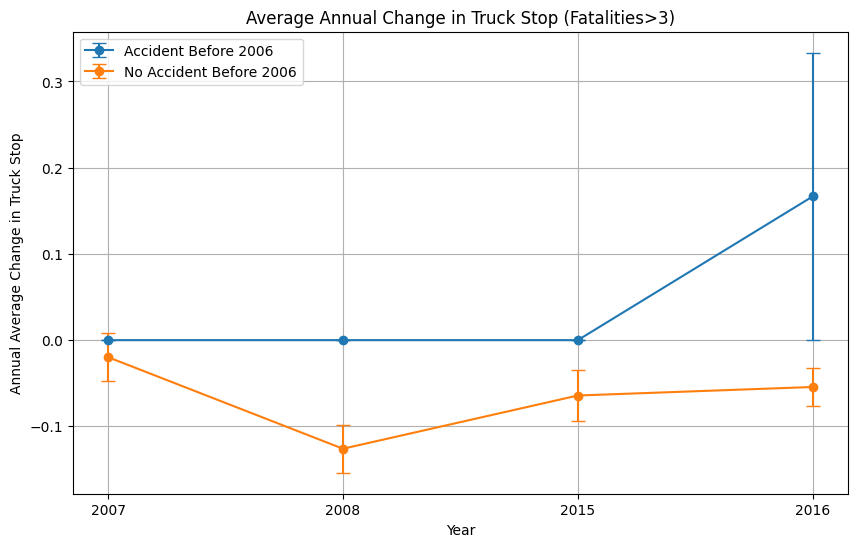
\includegraphics[width=4.6875in,height=\textheight]{images/output.png}

}

\caption{Parallel Trends Counties with accident Against without accident
before 2006}

\end{figure}%

\subsection{Parallel Trends Chart DID
Model}\label{sec-parallel-trends-chart-did-model}

\begin{figure}[H]

{\centering 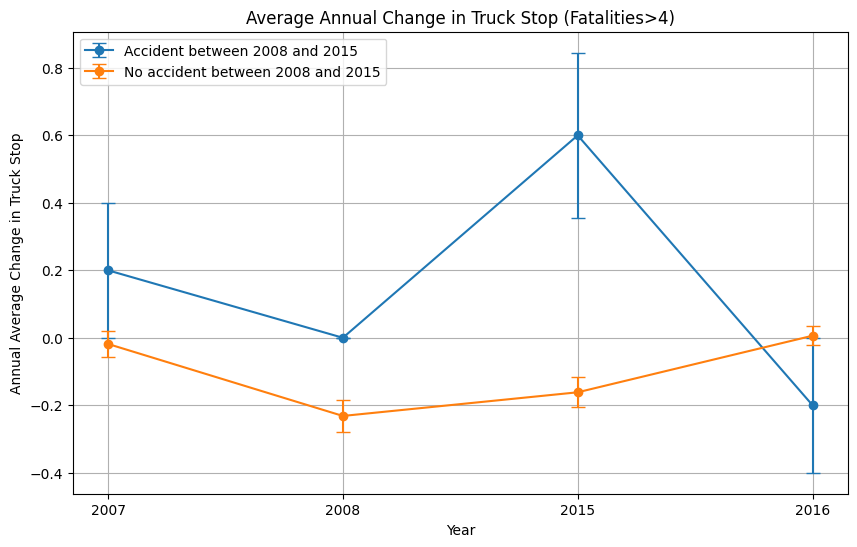
\includegraphics[width=4.71875in,height=\textheight]{images/output-01.png}

}

\caption{Parallel Trends Counties with accident Against without accident
between 2008 and 2015}

\end{figure}%


\renewcommand\refname{References}
  \bibliography{bibliography.bib}


\end{document}
